\documentclass[iutinfo,a4paper,10pt]{ustl-tdtp}
%\usepackage[utf8]{inputenc}  
%\usepackage[T1]{fontenc}
\usepackage{listings}  
\usepackage{version}
\usepackage{tikz}

%\usepackage[a4paper]{geometry}


\etablissement{\ustl}
\formation{DUT info 2ème année}
\matiere{Structures de données}
\titre{TD 6 : Arbres binaires de recherche (ABR)}
\date{\annee{2018}--\annee{2019}}
%\enseignant{}

%\includeversion{solution}
%\excludeversion{solution}

\newcommand{\case}{}%\rule[-.40cm]{0pt}{1cm}}
\newcommand{\ident}[3]{(\texttt{#1},~\texttt{#2},~\texttt{#3})}
\newcommand{\rien}{}

\parindent 0cm
\begin{document}
\maketitle
\thispagestyle{empty}

\subsection*{Exercice 1}
Énumérez tous les arbres binaires de recherche contenant les clés 1, 2, 3, 4.\\
\begin{solution}
{\color{red}
Il y a 14 arbres binaires de recherche distincts avec $n=4$, (Nombre de Catalan).
}
\end{solution}

\subsection*{Exercice 2}

Le professeur Ko\v smrlj pense avoir découvert une propriété remarquable des
arbres binaires de recherche. Supposez que la recherche d'une clef $k$ dans un
arbre binaire de recherche se termine sur une feuille. On considère trois
ensembles :
\begin{itemize}
\item $A$, les clés situées à gauche du chemin de recherche;
\item $B$, les clés situées sur le chemin de recherche;
\item $C$, les clés situées à droite du chemin de recherche.
\end{itemize}

Le professeur Ko\v smrlj affirme que, étant données trois clés, $a\in A$,
$b\in B$ et $c\in C$, quelconques, elles doivent satisfaire $a \leq b \leq c$.
Donnez un contre exemple qui soit le plus petit possible.

\begin{solution}
{\color{red}
En cherchant le n\oe ud 4 dans l'arbre ci-dessous, on a $A = \{2\}, B = \{1, 5 ,3, 4\}, C = \{6\}$.\\
\begin{tikzpicture}
	\node (is-root) {1}
		[sibling distance=2cm]
		child[missing]		
		child {
			child[missing]		
			node {5}
				[sibling distance=2cm]
				child { 
					node {3} 
				[sibling distance=2cm]
				child{ node {2} }	
				child { node {4} }		
				}	
				child { node {6} }		
		};
\end{tikzpicture}
}
\end{solution}


\subsection*{Exercice 3}
\begin{enumerate}

\item [a)] Écrivez une classe \texttt{BST} (pour \textit{Binary Search
    Tree}) avec une clé de type $T$, ses
  fils gauche et droit et ses constructeurs \texttt{BST<>()} et \texttt{BST<>(T key)}
  associés. 
\begin{solution}
{\color{red}
\begin{lstlisting}[language=Java]
public BST<T>{
  T key;
  BST<T> left, right;

  public BST(T key, BST<T> left, BST<T> right){
     this.key = key;
     this.left = left;
     this.right = right;
  }
  public BST(T key){
     this(key, new BST<T>(), new BST<T>());
  }
  public BST(){
     this(null, null, null);
  }
  
}
\end{lstlisting}
}
\end{solution}

\item [b)] Écrivez une méthode récursive \texttt{BST<T> bstMin()} qui
  retourne le sous-arbre de clé minimum de l'arbre, puis aussi la
  méthode \texttt{T min()}
\begin{solution}
{\color{red}
\begin{lstlisting}[language=Java]
protected BST<T> bstMin(){
  if (left.isEmpty()) 
    return this;
  return left.min();
}

public T min(){
    return bstMin().key;
}
\end{lstlisting}
}
\end{solution}

\item [c)] Quel est l'emplacement du successeur d'un n\oe ud dans un ABR? Décrivez tous les cas possibles.\\
\begin{solution}
{\color{red}
Le successeur d'un n\oe ud est la n\oe ud de clé minimum de son
sous-arbre droit. Si le n\oe ud d'origine n'a pas de fils droit alors il
s'agit du premier père droit rencontré en remontant la branche. Si le
fils droit du n\oe ud d'origine n'a pas de fils gauche alors il est
lui-même le successeur. Sinon le successeur est le dernier fils gauche
feuille du sous-arbre droit du n\oe ud d'origine.
}
\end{solution}
%\item [d)]Comment retrouver le successeur d'un n\oe ud à partir de la méthode \texttt{min}?

%\begin{solution}
%{\color{red}
%Il suffit donc d'appeler \texttt{ right.min()} sur le sous-arbre pour obtenir son
%successeur.
%}
%\end{solution}

\item [d)] Montrez que, si un n\oe ud d'un ABR (dont tous les n\oe uds sont distincts) a deux enfants, alors son successeur n'a pas de fils gauche et
 son prédécesseur n'a pas de fils droit.
 
\begin{solution}
{\color{red}
Son successeur est le minimum de son sous-arbre droit, donc le plus à gauche et respectivement pour le prédécesseur qui est le maximum de son sous-arbre gauche, donc le plus à droite.
}
 \end{solution}

\end{enumerate}


\subsection*{Exercice 4}

\begin{enumerate}
\item [a)] A partir d'un arbre binaire vide, ajoutez successivement les valeurs suivantes : 22, 09, 41, 39, 27, 06, 11, 45, 59, 18, 36.



\item [b)]Écrivez une méthode \texttt{boolean add(T key)},
  version récursive de l'algorithme d'ajout d'un n\oe ud de clé \texttt{key} dans un ABR.
\end{enumerate}

\begin{solution}
{\color{red}
\begin{lstlisting}[language=Java]
private BST<T> search(T key){
  if (isEmpty()) 
    return this;
  if (key.compareTo(value) > 0) 
    return left.search(key);
  if (key.compareTo(value) < 0) 
    return right.search(key);
  return this;
}

public boolean add(T key){
  BST<T> bst = search(key);
  if (!bst.isEmpty())
    return false;
  bst.copy(new BST<>(key));
  return true;
}
private void copy(BST<T> bst){
  key = bst.key;
  left = bst.left;
  right = bst.right;
}	
\end{lstlisting}

}
\end{solution}


\subsection*{Exercice 5}

\begin{enumerate}
\item [a)] A partir de l'arbre final de l'exercice précédent, supprimez successivement les valeurs 59 et 11. 
\item [b)] Supprimez maintenant les valeurs 22 et 41. Quelles valeurs choisissez-vous pour les remplacer? 

\begin{solution}
{\color{red}
Par leurs successeurs 27 et 45.
}
\end{solution}

\item [c)]  Écrivez une méthode récursive \texttt{T deleteMin()} qui supprime le n\oe ud de clé minimum de l'ABR.

\begin{solution}
{\color{red}
\begin{lstlisting}[language=Java]
private T deleteMin(){
    BST<T> bst = bstMin();
    T tmp = bst.key;
    bst.copy(bst.right);
    return tmp;
}

\end{lstlisting}
}
\end{solution}


\item [d)] Écrivez une méthode \texttt{delete(T key)}
  version récursive de l'algorithme de suppression d'un n\oe ud dans un ABR de racine $x$. Conseil : utilisez les méthodes \texttt{min} et \texttt{deleteMin} précédemment écrites.

\begin{solution}
{\color{red}
\begin{lstlisting}[language=Java]
public boolean delete(T key){
  BST<T> bst = search(key);
  if (bst.isEmpty())
    return false;
  if (bst.right.isEmpty)
    bst.copy(bst.left)
  else
    bst.key = bst.right.deleteMin();
  return true;
}

\end{lstlisting}
}
\end{solution}
\end{enumerate}

%\newpage
\subsection*{Exercice 6}

~\\ \textbf{Question 1:} Expliquez où se situe le prédécesseur d'un noeud dans
un arbre binaire de recherche. Détaillez votre réponse en fonction des
différentes configurations possibles.

\begin{solution}
{\color{red}
Si le noeud \emph{n} possède un fils gauche, le prédecesseur de \emph{n} est le maximum du sous arbre gauche.\\
	Si non, le prédecesseur est le premier parent gauche du noeud.}
\end{solution}

~\\ \textbf{Question 2:} À partir de l'arbre binaire de recherche
vide, ajoutez successivement les valeurs suivantes : 22, 7, 71, 39,
27, 2, 11, 42, 61, 18, 17. \textbf{Détaillez toutes les étapes !}\\

\begin{solution}
{\color{red}
Pour chaque insertion de valeurs, on part du noeud racine. \\
	Si la valeur est plus grande que la racine et que son fils droit est vide, on y insère la valeur. S'il y a un fils droit, on réitère avec le fils droit. \\
	Si la valeur est plus petite que la racine et que le fils gauche est vide, on y insère la valeur. S'il y a un fils gauche, on réitère avec le fils gauche.

\begin{center}
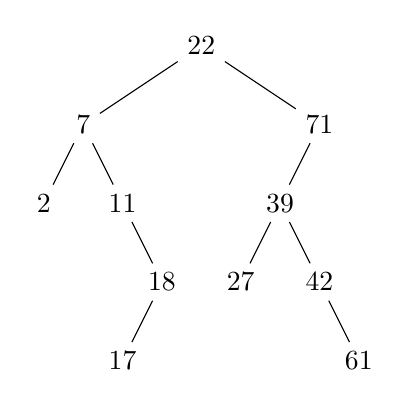
\begin{tikzpicture}[level distance=1cm,
level 1/.style={sibling distance=3cm},
level 2/.style={sibling distance=1cm}]
\node {22}
	child {node {7}
		child {node {2}}
		child {node {11}
			child[missing] {node {}}
			child{node{18}
				child{node{17}}
				child[missing] {node {}}
			}	
		}
	}
	child {node {71}
		child {node {39}
			child {node {27}}
			child {node {42}
				child[missing] {node {}}
				child {node {61}}
			}
		}
		child[missing] {node {}}
};
\end{tikzpicture}
\end{center}
}
\end{solution}

~\\ \textbf{Question 3:} Puis supprimez la valeur 22 en détaillant
aussi votre démarche.\\
\begin{solution}
{\color{red}
Soit on remplace 22 par son successeur (27), soit par son prédecesseur (18).

	\begin{center}
		\begin{tikzpicture}[level distance=1cm,
		level 1/.style={sibling distance=3cm},
		level 2/.style={sibling distance=1cm}]
		\node {27}
		child {node {7}
			child {node {2}}
			child {node {11}
				child[missing] {node {}}
				child{node{18}
					child{node{17}}
					child[missing] {node {}}
				}	
			}
		}
		child {node {71}
			child {node {39}
				child[missing] {node {}}
				child {node {42}
					child[missing] {node {}}
					child {node {61}}
				}
			}
			child[missing] {node {}}
		};
		\end{tikzpicture}
\hspace{3cm}
		\begin{tikzpicture}[level distance=1cm,
		level 1/.style={sibling distance=3cm},
		level 2/.style={sibling distance=1cm}]
		\node {18}
		child {node {7}
			child {node {2}}
			child {node {11}
				child[missing] {node {}}
				child{node{17}}	
			}
		}
		child {node {71}
			child {node {39}
				child {node {27}}
				child {node {42}
					child[missing] {node {}}
					child {node {61}}
				}
			}
			child[missing] {node {}}
		};
		\end{tikzpicture}
	\end{center}
}
\end{solution}

~\\ \textbf{Question 4:} Votre classe d'arbre binaire de recherche est
déclarée ainsi:
\begin{verbatim}
  public class BST<E> {
      E key;
      BST<E> left;
      BST<E> right;
  }
\end{verbatim}
Redéfinissez la fonction \texttt{equals} adaptée à votre classe
d'arbre de telle façon qu'elle retourne \texttt{true} si et seulement
si les deux arbres ont même structure et contiennent les mêmes
valeurs.

\begin{solution}
{\color{red}
\begin{lstlisting}[language=Java]
	public boolean equals(Object o) {
        if (o instanceof BST<?>) {
            BST<?> node = (BST<?>) o;
            if (value.equals(node.value)) {
                return true;
            }
            return ((left == null && node.left == null) || left.equals( node.left)) && 
                ((right == null && node.right == null) || right.equals( node.right));
        }
        return false;
    }
\end{lstlisting}
}
\end{solution}

\end{document}

